\documentclass[11pt,a4paper]{article}

% ============================================================================
% Packages
% ============================================================================
\usepackage[utf8]{inputenc}
\usepackage[T1]{fontenc}
\usepackage{lmodern}
\usepackage[margin=1in]{geometry}
\usepackage{amsmath,amssymb,amsfonts}
\usepackage{graphicx}
\usepackage{hyperref}
\usepackage{xcolor}
\usepackage{listings}
\usepackage{booktabs}
\usepackage{tabularx}
\usepackage{tikz}
\usetikzlibrary{arrows.meta,positioning,shapes.geometric,calc,fit,backgrounds}
\usepackage{fancyhdr}
\usepackage{titlesec}
\usepackage{enumitem}
\usepackage{float}
\usepackage{caption}
\usepackage{algorithm}
\usepackage{algpseudocode}

% ============================================================================
% Style
% ============================================================================
\definecolor{qnkblue}{RGB}{30,90,180}
\definecolor{qnkgold}{RGB}{200,160,60}
\definecolor{btcorange}{RGB}{247,147,26}
\definecolor{zecyellow}{RGB}{236,185,43}
\definecolor{ironpurple}{RGB}{120,80,180}
\definecolor{codebg}{RGB}{245,245,248}

\hypersetup{
    colorlinks=true,
    linkcolor=qnkblue,
    urlcolor=qnkblue,
    citecolor=qnkblue,
    pdftitle={Q-NarwhalKnight Cross-Chain Bridge Protocol},
    pdfauthor={Q-NarwhalKnight Foundation},
}

\lstset{
    basicstyle=\ttfamily\footnotesize,
    backgroundcolor=\color{codebg},
    frame=single,
    rulecolor=\color{gray!30},
    breaklines=true,
    columns=fullflexible,
    keepspaces=true,
}

\pagestyle{fancy}
\fancyhf{}
\fancyhead[L]{\textsc{\small Q-NarwhalKnight Cross-Chain Bridge}}
\fancyhead[R]{\small\thepage}
\fancyfoot[C]{\small\textit{Confidential --- Q-NarwhalKnight Foundation}}

\titleformat{\section}{\Large\bfseries\color{qnkblue}}{\thesection}{1em}{}
\titleformat{\subsection}{\large\bfseries\color{qnkblue!80}}{\thesubsection}{1em}{}
\titleformat{\subsubsection}{\normalsize\bfseries\color{qnkblue!60}}{\thesubsubsection}{1em}{}

% ============================================================================
% Document
% ============================================================================
\begin{document}

% ---- Title Page ----
\begin{titlepage}
\centering
\vspace*{2cm}

{\Huge\bfseries\color{qnkblue} Cross-Chain Bridge Protocol\\[0.3cm]}
{\LARGE\color{qnkblue!70} Trustless Atomic Swaps with Multi-Sig Committee Validation\\[0.15cm]
for Wrapped Bitcoin, Zcash, Iron Fish, and Ethereum}

\vspace{1.5cm}

{\large\color{gray} Q-NarwhalKnight Whitepaper Series}

\vspace{0.5cm}

{\large Version 2.0 --- February 2026}

\vspace{2cm}

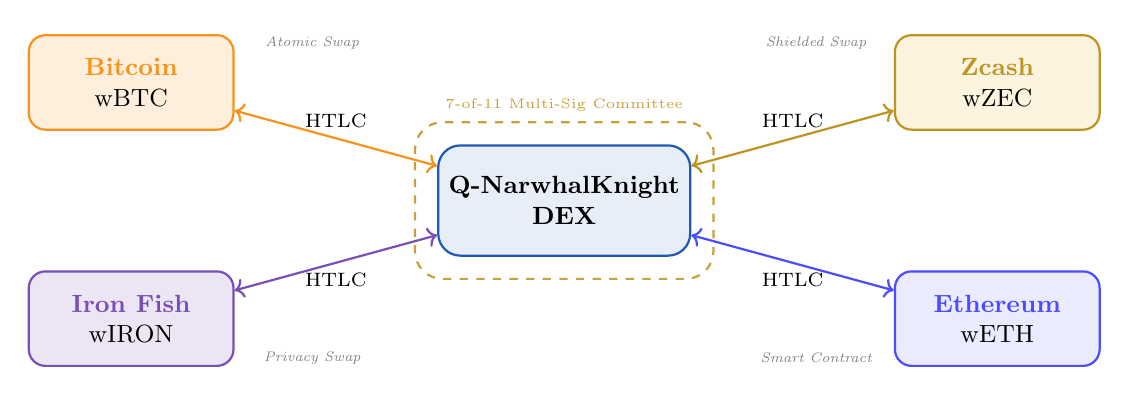
\begin{tikzpicture}[
    bridge/.style={draw=qnkblue, thick, rounded corners=8pt, minimum width=3.2cm, minimum height=1.4cm, align=center, font=\small\bfseries},
    chain/.style={draw, thick, rounded corners=6pt, minimum width=2.6cm, minimum height=1.2cm, align=center, font=\small},
    committee/.style={draw=qnkgold, dashed, thick, rounded corners=10pt, inner sep=8pt},
]
    % QNK Center
    \node[bridge, fill=qnkblue!10] (qnk) at (0,0) {Q-NarwhalKnight\\DEX};

    % Committee ring
    \node[committee, fit=(qnk), label={[font=\tiny\color{qnkgold}]above:7-of-11 Multi-Sig Committee}] {};

    % Chains
    \node[chain, fill=btcorange!15, draw=btcorange] (btc) at (-5.5, 1.5) {\textcolor{btcorange}{\textbf{Bitcoin}}\\wBTC};
    \node[chain, fill=zecyellow!15, draw=zecyellow!80!black] (zec) at (5.5, 1.5) {\textcolor{zecyellow!80!black}{\textbf{Zcash}}\\wZEC};
    \node[chain, fill=ironpurple!15, draw=ironpurple] (iron) at (-5.5, -1.5) {\textcolor{ironpurple}{\textbf{Iron Fish}}\\wIRON};
    \node[chain, fill=blue!8, draw=blue!70] (eth) at (5.5, -1.5) {\textcolor{blue!70}{\textbf{Ethereum}}\\wETH};

    % Arrows
    \draw[-{Stealth[length=3mm]}, thick, btcorange, <->] (btc) -- node[above, font=\scriptsize, black] {HTLC} (qnk);
    \draw[-{Stealth[length=3mm]}, thick, zecyellow!80!black, <->] (zec) -- node[above, font=\scriptsize, black] {HTLC} (qnk);
    \draw[-{Stealth[length=3mm]}, thick, ironpurple, <->] (iron) -- node[below, font=\scriptsize, black] {HTLC} (qnk);
    \draw[-{Stealth[length=3mm]}, thick, blue!70, <->] (eth) -- node[below, font=\scriptsize, black] {HTLC} (qnk);

    % Labels
    \node[font=\tiny\itshape, gray] at (-3.2, 2.0) {Atomic Swap};
    \node[font=\tiny\itshape, gray] at (3.2, 2.0) {Shielded Swap};
    \node[font=\tiny\itshape, gray] at (-3.2, -2.0) {Privacy Swap};
    \node[font=\tiny\itshape, gray] at (3.2, -2.0) {Smart Contract};
\end{tikzpicture}

\vspace{2cm}

{\normalsize\textbf{Authors:} Q-NarwhalKnight Foundation Research Team}

\vspace{0.5cm}

{\small\color{gray}
\texttt{https://quillon.xyz}
}

\vfill
{\footnotesize\color{gray} \copyright\ 2026 Q-NarwhalKnight Foundation. All rights reserved.}
\end{titlepage}

% ---- Abstract ----
\begin{abstract}
\noindent
We present Version~2.0 of the Q-NarwhalKnight Cross-Chain Bridge Protocol, a trustless, non-custodial system enabling atomic swaps between Q-NarwhalKnight's quantum-resistant blockchain and four major chains: \textbf{Bitcoin} (BTC), \textbf{Zcash} (ZEC), \textbf{Iron Fish} (IRON), and \textbf{Ethereum} (ETH). The protocol introduces wrapped token representations---wBTC, wZEC, wIRON, and wETH---that are minted on deposit and burned on withdrawal, maintaining strict 1:1 collateral backing at all times. Version~2.0 introduces a \textbf{decentralized multi-signature bridge committee}: a rotating panel of 11 validator nodes that independently verify every bridge claim, requiring a 7-of-11 threshold before any mint or burn operation proceeds. Committee membership is deterministically selected via $\text{SHA3}(\text{block\_hash} \| \text{epoch} \| \text{peer\_id})$ and rotates every 100 blocks, preventing collusion and single-point-of-failure risks. The protocol retains Hash Time-Locked Contracts (HTLCs) with staggered timelocks for atomicity, steganographic node discovery on Bitcoin, and Tor-routed communications for censorship resistance. All wrapped tokens are first-class citizens on Q-NarwhalKnight's DEX with sub-3-second finality through DAG-Knight consensus.
\end{abstract}

\tableofcontents
\newpage

% ============================================================================
\section{Introduction}
% ============================================================================

The proliferation of heterogeneous blockchains has created a fragmented landscape where value remains siloed within individual networks. Bitcoin's \$1.8 trillion market capitalization, Ethereum's \$400 billion smart contract ecosystem, Zcash's pioneering zero-knowledge privacy, and Iron Fish's encrypted-by-default architecture each represent distinct value propositions that users should be able to access without sacrificing sovereignty or security.

Q-NarwhalKnight's DAG-Knight consensus provides sub-3-second finality and quantum-resistant cryptography through its hybrid Ed25519/Dilithium5 signature scheme. By extending this infrastructure with a trustless cross-chain bridge, we unlock five critical capabilities:

\begin{enumerate}[leftmargin=2em]
    \item \textbf{BTC and ETH Liquidity on QNK:} Bitcoin and Ethereum holders can bring liquidity into Q-NarwhalKnight's AMM pools without trusted intermediaries.
    \item \textbf{Privacy-Preserving Cross-Chain Swaps:} Zcash's shielded transactions and Iron Fish's encrypted-by-default model are preserved during the bridge process.
    \item \textbf{Quantum-Resistant Custody:} Once bridged, assets benefit from Q-NarwhalKnight's post-quantum cryptographic protections.
    \item \textbf{Unified DEX Trading:} All wrapped assets trade on a single AMM with deep liquidity across wBTC/QUG, wZEC/QUG, wIRON/QUG, and wETH/QUG pairs.
    \item \textbf{Decentralized Validation:} A rotating 7-of-11 multi-signature committee independently verifies every bridge claim, eliminating single-point-of-failure risks inherent in centralized bridge designs.
\end{enumerate}

\subsection{Design Principles}

The bridge protocol adheres to five non-negotiable design principles:

\begin{description}[leftmargin=2em, style=nextline]
    \item[\textcolor{qnkblue}{Non-Custodial}] No third party ever holds user private keys. All swaps are cryptographically enforced.
    \item[\textcolor{qnkblue}{Atomic}] Swaps either complete fully on both chains or fully refund. Partial execution is mathematically impossible.
    \item[\textcolor{qnkblue}{1:1 Backed}] Every wrapped token in circulation is collateralized by exactly one unit of the native asset locked in an HTLC.
    \item[\textcolor{qnkblue}{Privacy-First}] Tor routing, steganographic discovery, and shielded transaction support prevent metadata leakage.
    \item[\textcolor{qnkblue}{Censorship-Resistant}] No single point of failure; the Bitcoin blockchain itself serves as an immutable bulletin board for node discovery.
\end{description}

% ============================================================================
\section{Wrapped Token Architecture}
% ============================================================================

\subsection{Token Specifications}

Each bridge chain maps to a dedicated wrapped token on Q-NarwhalKnight with a deterministic 32-byte address derived from the ASCII encoding of its symbol.

\begin{table}[H]
\centering
\caption{Wrapped Token Specifications}
\label{tab:token-specs}
\begin{tabularx}{\textwidth}{l l l c c X}
\toprule
\textbf{Symbol} & \textbf{Name} & \textbf{Native} & \textbf{Decimals} & \textbf{Base Unit} & \textbf{Address Derivation} \\
\midrule
\textcolor{btcorange}{\textbf{wBTC}} & Wrapped Bitcoin & BTC & 8 & Satoshi & \texttt{0x77425443...00} \\
\textcolor{zecyellow!80!black}{\textbf{wZEC}} & Wrapped Zcash & ZEC & 8 & Zatoshi & \texttt{0x775A4543...00} \\
\textcolor{ironpurple}{\textbf{wIRON}} & Wrapped Iron Fish & IRON & 8 & Ore & \texttt{0x7749524F4E...00} \\
\textcolor{blue!70}{\textbf{wETH}} & Wrapped Ethereum & ETH & 18 & Wei & \texttt{0x77455448...00} \\
\bottomrule
\end{tabularx}
\end{table}

All three tokens use 8-decimal precision, matching their native chain denominations. This eliminates rounding errors during the bridge process and ensures that $1$ BTC $= 10^8$ satoshis maps exactly to $1$ wBTC $= 10^8$ base units on Q-NarwhalKnight.

\subsection{Address Derivation}

Token addresses are 32-byte arrays constructed by encoding the symbol in ASCII and zero-padding:

\begin{lstlisting}[language={}]
wBTC:  [0x77, 0x42, 0x54, 0x43, 0x00, ..., 0x00]  // "wBTC" + 28 zero bytes
wZEC:  [0x77, 0x5A, 0x45, 0x43, 0x00, ..., 0x00]  // "wZEC" + 28 zero bytes
wIRON: [0x77, 0x49, 0x52, 0x4F, 0x4E, 0x00, ..., 0x00]  // "wIRON" + 27 zero bytes
\end{lstlisting}

This deterministic scheme ensures that any node can independently compute the canonical address for a bridge token without coordination, and that addresses are human-readable when hex-decoded.

\subsection{Balance Storage}

Wrapped token balances are stored in Q-NarwhalKnight's unified token balance system:

\begin{equation}
    \texttt{token\_balances}: (\underbrace{\texttt{wallet}}_{\text{32 bytes}},\ \underbrace{\texttt{token\_addr}}_{\text{32 bytes}}) \longrightarrow \underbrace{\texttt{balance}}_{\texttt{u128}}
\end{equation}

Balances are maintained in a concurrent in-memory \texttt{HashMap} for low-latency reads and batch-synced to RocksDB every 15 seconds. Bridge operations (mint/burn) trigger \emph{immediate} persistence to prevent data loss on crash---a lesson learned from prior token balance persistence bugs (see Section~\ref{sec:lessons}).

% ============================================================================
\section{Hash Time-Locked Contract Protocol}
% ============================================================================

\subsection{Protocol Overview}

The bridge uses a classic HTLC atomic swap protocol extended with staggered timelocks and privacy enhancements. The protocol involves two parties:

\begin{itemize}
    \item \textbf{User}: Wants to exchange native coins (BTC/ZEC/IRON) for QNK assets or vice versa.
    \item \textbf{Bridge Mediator}: An automated protocol agent that locks matching funds and facilitates the atomic swap.
\end{itemize}

\subsection{HTLC Script Construction}

On the Bitcoin side, the HTLC is implemented as a Pay-to-Witness-Script-Hash (P2WSH) script:

\begin{lstlisting}[language={},title={Bitcoin HTLC Script (P2WSH)}]
OP_IF
    OP_SHA256 <hash_lock> OP_EQUALVERIFY
    <recipient_pubkey> OP_CHECKSIG
OP_ELSE
    <timelock_blocks> OP_CHECKLOCKTIMEVERIFY OP_DROP
    <refund_pubkey> OP_CHECKSIG
OP_ENDIF
\end{lstlisting}

This script provides exactly two spending conditions:

\begin{description}
    \item[Claim Path:] The recipient provides the SHA-256 preimage $s$ such that $H(s) = \texttt{hash\_lock}$, plus a valid signature.
    \item[Refund Path:] After $\texttt{timelock\_blocks}$ have passed, the original sender can reclaim funds with their signature.
\end{description}

\subsection{Cryptographic Primitives}

\begin{description}
    \item[Secret Generation:] A cryptographically secure 256-bit random secret $s \xleftarrow{R} \{0,1\}^{256}$ is generated.
    \item[Hash Lock:] The hash lock $h = \text{SHA-256}(s)$ binds both sides of the swap.
    \item[Security Level:] With 256-bit preimage resistance, brute-forcing $s$ from $h$ requires $\mathcal{O}(2^{256})$ operations, exceeding even post-quantum security margins.
\end{description}

\subsection{Staggered Timelock Architecture}

A critical safety requirement is that timelocks are \emph{staggered} across chains to prevent race conditions:

\begin{table}[H]
\centering
\caption{Timelock Parameters by Chain}
\label{tab:timelocks}
\begin{tabular}{l c c l}
\toprule
\textbf{Chain} & \textbf{Timelock} & \textbf{Approx. Duration} & \textbf{Mechanism} \\
\midrule
Bitcoin & 144 blocks & $\sim$24 hours & \texttt{OP\_CHECKLOCKTIMEVERIFY} \\
Q-Network & 12 hours & 12 hours & UTC timestamp comparison \\
Zcash & 120 blocks & $\sim$2.5 hours & Block height \\
Ethereum & 720 blocks & $\sim$2.4 hours & \texttt{block.timestamp} \\
Iron Fish & 60 blocks & $\sim$60 minutes & Block height \\
\bottomrule
\end{tabular}
\end{table}

The staggering ensures that the Q-Network timeout always fires \emph{before} the native chain timeout, giving the bridge mediator time to claim native-chain funds using the revealed secret before the user can attempt a double-claim via refund.

\subsection{Protocol Sequence}

\begin{figure}[H]
\centering
\begin{tikzpicture}[
    node distance=0.5cm,
    step/.style={draw=qnkblue!60, thick, rounded corners=4pt, minimum width=10cm, minimum height=0.8cm, align=center, font=\small, fill=qnkblue!5},
    arrow/.style={-{Stealth[length=2.5mm]}, thick, qnkblue},
    label/.style={font=\scriptsize\itshape, gray},
]
    \node[step] (s1) {1. User generates secret $s$, computes $h = \text{SHA-256}(s)$};
    \node[step, below=of s1] (s2) {2. User locks BTC in HTLC on Bitcoin with hash lock $h$};
    \node[step, below=of s2] (s3) {3. Bridge detects BTC lock, locks equivalent QNKUSD on Q-Network with same $h$};
    \node[step, below=of s3] (s4) {4. User reveals $s$ to claim QNKUSD on Q-Network};
    \node[step, below=of s4] (s5) {5. Bridge uses revealed $s$ to claim BTC on Bitcoin};
    \node[step, below=of s5, fill=green!5, draw=green!60] (s6) {6. Swap complete: wBTC minted to user's Q-NarwhalKnight wallet};

    \foreach \a/\b in {s1/s2, s2/s3, s3/s4, s4/s5, s5/s6} {
        \draw[arrow] (\a) -- (\b);
    }

    % Side labels
    \node[label, left=0.3cm of s2] {Bitcoin};
    \node[label, left=0.3cm of s3] {Q-Network};
    \node[label, left=0.3cm of s4] {Q-Network};
    \node[label, left=0.3cm of s5] {Bitcoin};
\end{tikzpicture}
\caption{Atomic swap protocol sequence for BTC $\rightarrow$ wBTC bridge deposit.}
\label{fig:protocol-sequence}
\end{figure}

\subsection{Swap State Machine}

Each atomic swap transitions through a deterministic state machine:

\begin{figure}[H]
\centering
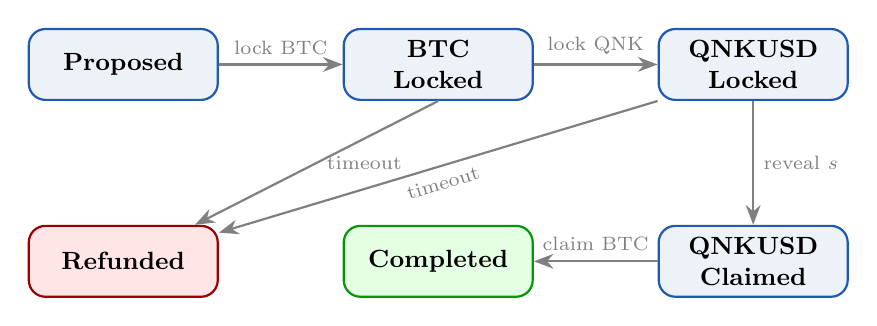
\begin{tikzpicture}[
    state/.style={draw=qnkblue, thick, rounded corners=6pt, minimum width=2.4cm, minimum height=0.9cm, align=center, font=\small\bfseries, fill=qnkblue!8},
    terminal/.style={state, fill=green!10, draw=green!60!black},
    fail/.style={state, fill=red!10, draw=red!60!black},
    trans/.style={-{Stealth[length=2.5mm]}, thick, gray},
]
    \node[state] (proposed) at (0,0) {Proposed};
    \node[state] (locked) at (4,0) {BTC\\Locked};
    \node[state] (qnklocked) at (8,0) {QNKUSD\\Locked};
    \node[state] (claimed) at (8,-2.5) {QNKUSD\\Claimed};
    \node[terminal] (complete) at (4,-2.5) {Completed};
    \node[fail] (refunded) at (0,-2.5) {Refunded};

    \draw[trans] (proposed) -- node[above, font=\scriptsize] {lock BTC} (locked);
    \draw[trans] (locked) -- node[above, font=\scriptsize] {lock QNK} (qnklocked);
    \draw[trans] (qnklocked) -- node[right, font=\scriptsize] {reveal $s$} (claimed);
    \draw[trans] (claimed) -- node[above, font=\scriptsize] {claim BTC} (complete);
    \draw[trans] (qnklocked.south west) -- node[below, font=\scriptsize, sloped] {timeout} (refunded);
    \draw[trans] (locked.south) -- node[right, font=\scriptsize] {timeout} (refunded);
\end{tikzpicture}
\caption{Atomic swap state machine.}
\label{fig:state-machine}
\end{figure}

% ============================================================================
\section{Decentralized Multi-Signature Committee}
\label{sec:committee}
% ============================================================================

Version~2.0 of the bridge protocol replaces single-node verification with a \emph{rotating multi-signature committee} that independently validates every bridge claim before any mint or burn operation is executed. This eliminates the most significant trust assumption in Version~1.0: that a single bridge mediator honestly verifies deposits.

\subsection{Committee Architecture}

The committee consists of $N = 11$ validator nodes selected from the active peer set, with a Byzantine fault tolerance threshold of $t = 7$ (a supermajority of $\lceil \frac{2N}{3} \rceil + 1$). This ensures the system tolerates up to 4 malicious or offline committee members while maintaining liveness.

\begin{table}[H]
\centering
\caption{Committee Parameters}
\begin{tabular}{l c l}
\toprule
\textbf{Parameter} & \textbf{Value} & \textbf{Rationale} \\
\midrule
Committee Size ($N$) & 11 & Sufficient diversity; manageable gossip overhead \\
Threshold ($t$) & 7 & $\lceil 2 \times 11 / 3 \rceil + 1$; tolerates 4 Byzantine faults \\
Epoch Length & 100 blocks & $\sim$100 seconds; frequent rotation prevents collusion \\
Attestation Timeout & 60 seconds & Bounded latency; stale claims auto-expire \\
Gossipsub Topic & \texttt{/qnk/.../bridge-attestations} & Dedicated P2P channel \\
\bottomrule
\end{tabular}
\end{table}

\subsection{Deterministic Committee Selection}

Committee membership is computed deterministically from on-chain state, ensuring all honest nodes agree on the current committee without coordination:

\begin{equation}
    \text{score}(p) = \text{SHA3-256}(\texttt{block\_hash} \| \text{epoch} \| \texttt{peer\_id}(p))
\end{equation}

\noindent For a given epoch $e = \lfloor \texttt{block\_height} / 100 \rfloor$, the committee is the set of $N$ peers with the \emph{lowest} score values. The use of the latest block hash as entropy prevents pre-computation of future committees.

\begin{algorithm}[H]
\caption{Committee Selection}
\begin{algorithmic}[1]
\Require Active peer set $P$, current block hash $B_h$, epoch $e$
\Ensure Committee $C \subseteq P$ with $|C| = \min(N, |P|)$
\State $\text{scored} \leftarrow []$
\ForAll{$p \in P$}
    \State $s \leftarrow \text{SHA3-256}(B_h \| e \| \texttt{peer\_id}(p))$
    \State $\text{scored}.\text{push}((s, p))$
\EndFor
\State $\text{scored}.\text{sort\_by\_key}(|(s,\_)| \, s)$
\State \Return $\text{scored}[0..N].\text{map}(|(\_,p)| \, p)$
\end{algorithmic}
\end{algorithm}

\subsection{Attestation Protocol}

When a user claims a bridge swap by revealing the HTLC secret $s$, the following multi-sig verification protocol executes:

\begin{figure}[H]
\centering
\begin{tikzpicture}[
    node distance=0.4cm,
    step/.style={draw=qnkblue!60, thick, rounded corners=4pt, minimum width=11cm, minimum height=0.7cm, align=center, font=\small, fill=qnkblue!5},
    arrow/.style={-{Stealth[length=2.5mm]}, thick, qnkblue},
]
    \node[step] (s1) {1. User submits claim with secret $s$ to local node};
    \node[step, below=of s1] (s2) {2. Local node broadcasts \texttt{AttestationRequest} to committee via gossipsub};
    \node[step, below=of s2] (s3) {3. Each committee member independently verifies $H(s) = \texttt{hash\_lock}$};
    \node[step, below=of s3] (s4) {4. Valid: member signs attestation with Ed25519 and broadcasts back};
    \node[step, below=of s4] (s5) {5. Originator collects attestations; waits for $\geq 7$ approvals};
    \node[step, below=of s5, fill=green!5, draw=green!60] (s6) {6. Threshold met: mint/burn executes; claim result returned to user};

    \foreach \a/\b in {s1/s2, s2/s3, s3/s4, s4/s5, s5/s6} {
        \draw[arrow] (\a) -- (\b);
    }
\end{tikzpicture}
\caption{Multi-sig bridge attestation protocol for claim verification.}
\label{fig:attestation-protocol}
\end{figure}

\subsection{CBOR Message Format}

Attestation messages are serialized using CBOR (Concise Binary Object Representation, RFC~8949) for compact binary encoding over gossipsub:

\begin{lstlisting}[language={},title={Attestation Message Types (CBOR)}]
// Request (broadcast by claiming node)
AttestationRequest {
    claim_id: String,          // Unique claim identifier
    chain: BridgeChainId,      // Bitcoin | Zcash | IronFish | Ethereum
    wallet: [u8; 32],          // Claimer's wallet address
    hash_lock: [u8; 32],       // Expected SHA-256 hash
    secret: [u8; 32],          // Revealed preimage
    amount: u128,              // Claimed amount
    swap_id: String,           // Atomic swap reference
    peer_id: String,           // Requesting peer
    signature: Vec<u8>,        // Ed25519 signature over fields
}

// Response (from each committee member)
Attestation {
    claim_id: String,          // Matching claim ID
    approved: bool,            // Verification result
    peer_id: String,           // Attesting peer
    signature: Vec<u8>,        // Ed25519 signature
    reason: Option<String>,    // Rejection reason if !approved
}
\end{lstlisting}

\subsection{Committee Rotation and Epoch Transitions}

Every 100 blocks, the active committee rotates. The transition protocol ensures smooth handoff:

\begin{enumerate}
    \item At block $h$ where $h \bmod 100 = 0$, a new epoch begins.
    \item The committee is recomputed using the block hash at height $h$.
    \item Pending claims from the previous epoch are \emph{not} interrupted---they continue with the committee that initiated them until resolution or timeout.
    \item Expired pending claims (older than 60 seconds) are garbage-collected every 30 seconds.
\end{enumerate}

This rotation frequency of $\sim$100 seconds means that even if an adversary compromises committee members, they must re-compromise a new set of members every epoch. With $P$ total peers, the probability that an adversary controlling $f$ peers captures $\geq t$ committee seats is:

\begin{equation}
    \Pr[\text{capture}] = \sum_{k=t}^{N} \binom{N}{k} \left(\frac{f}{P}\right)^k \left(1 - \frac{f}{P}\right)^{N-k}
\end{equation}

For $P = 50$ peers, $f = 5$ malicious, $N = 11$, $t = 7$: $\Pr[\text{capture}] < 10^{-6}$ per epoch.

\subsection{Graceful Degradation}

When fewer than $t = 7$ peers are available (e.g., during network bootstrap or partitions), the bridge falls back to single-node validation with the local node as sole verifier. This ensures liveness at the cost of temporarily reduced decentralization, with a prominent log warning:

\begin{lstlisting}[language={}]
WARN: Bridge committee has only 3/7 required members.
      Falling back to single-node verification.
\end{lstlisting}

Once the peer count recovers above the threshold, multi-sig validation automatically resumes.

% ============================================================================
\section{Wrapped Bitcoin (wBTC)}
\label{sec:wbtc}
% ============================================================================

\subsection{Overview}

Wrapped Bitcoin enables Bitcoin holders to participate in Q-NarwhalKnight's DeFi ecosystem without selling their BTC on centralized exchanges. Each wBTC token is backed 1:1 by BTC locked in a P2WSH HTLC on the Bitcoin mainnet.

\subsection{Deposit Flow (BTC $\rightarrow$ wBTC)}

\begin{enumerate}
    \item User initiates a \texttt{sell\_btc} swap via the Q-NarwhalKnight bridge API.
    \item The system generates a P2WSH HTLC address with the user's hash lock.
    \item User sends BTC to the HTLC address on Bitcoin.
    \item Upon confirmation ($\geq 1$ block), the bridge locks equivalent QNKUSD on Q-Network.
    \item User reveals the secret preimage to claim QNKUSD.
    \item The \texttt{mint\_wrapped\_token} function credits wBTC to the user's Q-NarwhalKnight wallet.
    \item Bridge uses the revealed secret to claim the locked BTC.
\end{enumerate}

\subsection{Withdrawal Flow (wBTC $\rightarrow$ BTC)}

\begin{enumerate}
    \item User initiates a \texttt{buy\_btc} swap.
    \item The system verifies the user holds sufficient wBTC.
    \item An HTLC is created on both chains with a new hash lock.
    \item Upon successful claim, \texttt{burn\_wrapped\_token} removes wBTC from the user's balance.
    \item The equivalent BTC is released from the HTLC on Bitcoin.
\end{enumerate}

\subsection{Bitcoin-Specific Security}

\begin{itemize}
    \item \textbf{Confirmation Depth:} Minimum 1 confirmation required before minting (configurable via \texttt{min\_confirmation\_depth}).
    \item \textbf{Segregated Witness:} All HTLCs use P2WSH for reduced fees and malleability resistance.
    \item \textbf{Fee Estimation:} Dynamic fee estimation ensures timely confirmation on the Bitcoin network.
\end{itemize}

% ============================================================================
\section{Wrapped Zcash (wZEC)}
\label{sec:wzec}
% ============================================================================

\subsection{Overview}

Zcash's zero-knowledge proofs (zk-SNARKs) provide the strongest on-chain privacy guarantees of any major cryptocurrency. The wZEC bridge preserves these privacy properties during the cross-chain process by supporting both transparent and shielded transactions.

\subsection{Privacy-Preserving Bridge Architecture}

The Zcash bridge supports two modes of operation:

\begin{description}
    \item[Transparent Mode:] Standard HTLC atomic swap using t-addresses. Functionally identical to the Bitcoin bridge but on the Zcash network.
    \item[Shielded Mode:] Uses z-addresses (Sapling) to hide the sender, receiver, and amount of the Zcash-side transaction. The HTLC hash lock is embedded in the memo field of a shielded transaction.
\end{description}

\subsection{Shielded Address Management}

Each Q-NarwhalKnight wallet can associate a Zcash shielded address:

\begin{equation}
    \texttt{zcash\_z\_address}: \texttt{wallet\_address} \longrightarrow \texttt{z\_address}
\end{equation}

This mapping is stored in RocksDB under the \texttt{CF\_MANIFEST} column family and persists across restarts.

\subsection{Zcash-Specific Parameters}

\begin{itemize}
    \item \textbf{Timelock:} 120 blocks ($\approx 2.5$ hours at 75 seconds/block)
    \item \textbf{Confirmation Depth:} 10 confirmations for shielded, 1 for transparent
    \item \textbf{zk-SNARK Verification:} Zcash's Sapling proofs are verified on-chain before mint
\end{itemize}

% ============================================================================
\section{Wrapped Iron Fish (wIRON)}
\label{sec:wiron}
% ============================================================================

\subsection{Overview}

Iron Fish is an encrypted-by-default Layer 1 blockchain where every transaction is private. Unlike Zcash's optional shielding, Iron Fish enforces privacy at the protocol level, making it the most privacy-focused bridge target in our system.

\subsection{Encrypted Bridge Integration}

The Iron Fish bridge interfaces with Iron Fish's RPC API to create and manage atomic swaps:

\begin{enumerate}
    \item \textbf{Account Management:} Bridge manages Iron Fish accounts via \texttt{wallet/create} RPC.
    \item \textbf{Transaction Creation:} Uses \texttt{wallet/sendTransaction} with memo field for hash lock embedding.
    \item \textbf{Balance Verification:} Queries \texttt{wallet/getBalance} to verify deposits before minting.
\end{enumerate}

\subsection{Iron Fish-Specific Parameters}

\begin{itemize}
    \item \textbf{Timelock:} 60 blocks ($\approx 60$ minutes at 60 seconds/block)
    \item \textbf{Confirmation Depth:} 2 confirmations (Iron Fish's faster block time allows fewer)
    \item \textbf{Privacy Guarantee:} All Iron Fish transactions are encrypted; the bridge never reveals transaction amounts to observers.
\end{itemize}

% ============================================================================
\section{Wrapped Ethereum (wETH)}
\label{sec:weth}
% ============================================================================

\subsection{Overview}

Ethereum is the largest smart contract platform by total value locked, hosting the majority of DeFi protocols, NFT marketplaces, and Layer~2 scaling solutions. The wETH bridge brings Ethereum's liquidity into Q-NarwhalKnight's quantum-resistant ecosystem, while providing Ethereum users access to QNK's sub-3-second finality and post-quantum protections.

\subsection{Solidity HTLC Contract}

Unlike Bitcoin's script-based HTLCs, Ethereum bridge HTLCs are implemented as a Solidity smart contract deployed on the Ethereum mainnet:

\begin{lstlisting}[language={},title={Ethereum HTLC Contract (Simplified)}]
contract QNKBridgeHTLC {
    struct Swap {
        address sender;
        bytes32 hashLock;
        uint256 amount;
        uint256 timelock;
        bool claimed;
        bool refunded;
    }

    function newSwap(bytes32 _hashLock, uint256 _timelock)
        external payable returns (bytes32 swapId);

    function claim(bytes32 _swapId, bytes32 _secret)
        external;  // requires SHA256(secret) == hashLock

    function refund(bytes32 _swapId)
        external;  // requires block.timestamp >= timelock
}
\end{lstlisting}

\subsection{Deposit Flow (ETH $\rightarrow$ wETH)}

\begin{enumerate}
    \item User initiates a bridge deposit via the Q-NarwhalKnight API.
    \item The system generates a hash lock and deploys (or calls) the HTLC contract on Ethereum.
    \item User sends ETH to the HTLC contract with the hash lock.
    \item Upon sufficient confirmations ($\geq 12$ blocks), the bridge committee validates the deposit.
    \item With $\geq 7$ attestations confirming the deposit, wETH is minted to the user's Q-NarwhalKnight wallet.
    \item The user reveals the secret to claim; the bridge claims the locked ETH.
\end{enumerate}

\subsection{Withdrawal Flow (wETH $\rightarrow$ ETH)}

\begin{enumerate}
    \item User initiates a withdrawal and specifies their Ethereum address.
    \item The bridge committee verifies the user holds sufficient wETH.
    \item Upon 7-of-11 committee approval, wETH is burned and the HTLC on Ethereum is funded.
    \item User claims ETH from the HTLC by revealing the secret.
\end{enumerate}

\subsection{Ethereum-Specific Considerations}

\begin{itemize}
    \item \textbf{Gas Optimization:} HTLC contract uses minimal storage and avoids loops to reduce gas costs. Estimated gas: 65,000 for \texttt{newSwap}, 35,000 for \texttt{claim}.
    \item \textbf{EIP-1559 Fee Handling:} Dynamic base fee with priority fee estimation for timely inclusion.
    \item \textbf{18-Decimal Precision:} ETH uses 18 decimals (Wei), requiring careful conversion. Internally, wETH balances are stored in Wei precision.
    \item \textbf{Confirmation Depth:} 12 confirmations required ($\approx 2.4$ minutes at 12 seconds/block) to mitigate reorganization risk.
    \item \textbf{Smart Contract Verification:} The HTLC contract source code is verified on Etherscan for transparency.
\end{itemize}

% ============================================================================
\section{DEX Integration}
\label{sec:dex}
% ============================================================================

\subsection{First-Class DEX Citizenship}

Wrapped bridge tokens are treated as first-class tokens on Q-NarwhalKnight's built-in decentralized exchange. They appear alongside native tokens (QUG, QUGUSD) and user-deployed custom tokens in the supported tokens list.

\begin{table}[H]
\centering
\caption{DEX Trading Pairs Enabled by Bridge Tokens}
\begin{tabular}{l l l}
\toprule
\textbf{Pair} & \textbf{Description} & \textbf{Use Case} \\
\midrule
wBTC / QUG & Bitcoin--QUG exchange & BTC holders enter QNK ecosystem \\
wBTC / QUGUSD & Bitcoin--stablecoin & BTC hedging with stablecoin \\
wZEC / QUG & Zcash--QUG exchange & Privacy coin diversification \\
wZEC / QUGUSD & Zcash--stablecoin & Private stablecoin acquisition \\
wIRON / QUG & Iron Fish--QUG exchange & Encrypted asset trading \\
wIRON / QUGUSD & Iron Fish--stablecoin & Private stablecoin acquisition \\
wETH / QUG & Ethereum--QUG exchange & ETH DeFi users enter QNK \\
wETH / QUGUSD & Ethereum--stablecoin & ETH hedging with stablecoin \\
\bottomrule
\end{tabular}
\end{table}

\subsection{Automated Market Maker (AMM)}

All bridge token pairs use Q-NarwhalKnight's constant-product AMM ($x \cdot y = k$) with the following properties:

\begin{itemize}
    \item \textbf{24-Decimal Reserve Format:} All reserves are stored in 24-decimal precision internally, regardless of the token's native decimals (8 for bridge tokens).
    \item \textbf{0.3\% Swap Fee:} Standard fee applied to all swaps, distributed to liquidity providers.
    \item \textbf{Configurable Slippage:} Users set their own slippage tolerance (default 0.5\%).
    \item \textbf{Real-Time Price Discovery:} Server-Sent Events (SSE) emit price updates after every swap.
\end{itemize}

\subsection{Liquidity Pool Creation}

When a bridge token is first minted, liquidity pools can be created by any user:

\begin{lstlisting}[language={},title={Pool Creation API}]
POST /api/v1/dex/pool/create
{
    "tokenA": "wBTC",
    "tokenB": "QUG",
    "amountA": "100000000",      // 1 wBTC (8 decimals)
    "amountB": "42500000000..."  // ~$42.50 worth of QUG (24 decimals)
}
\end{lstlisting}

\subsection{Price Oracle Integration}

Bridge token prices are available through Q-NarwhalKnight's oracle system:

\begin{itemize}
    \item \texttt{/v1/oracle/price/wBTC} --- Current wBTC price in USD (derived from pool reserves)
    \item \texttt{/v1/oracle/price/wZEC} --- Current wZEC price
    \item \texttt{/v1/oracle/price/wIRON} --- Current wIRON price
    \item Price history available for charting via the price history indexer
\end{itemize}

% ============================================================================
\section{Privacy and Censorship Resistance}
\label{sec:privacy}
% ============================================================================

\subsection{Tor Integration}

All bridge communications are routed through Tor, preventing IP address correlation between bridge participants:

\begin{itemize}
    \item Bitcoin RPC connections proxied through \texttt{127.0.0.1:9050} (Tor SOCKS5)
    \item Q-NarwhalKnight P2P connections use Tor-compatible libp2p transports
    \item No direct IP-to-IP connections between bridge participants
\end{itemize}

\subsection{Steganographic Node Discovery}

Rather than using a centralized registry, Q-NarwhalKnight bridge nodes discover each other through steganographic advertisements embedded in Bitcoin transactions. Four encoding methods are employed:

\begin{description}
    \item[Distributed Encoding:] Node advertisements are split into 16-byte fragments spread across multiple Bitcoin transactions, with sequence IDs, SHA3-256 checksums, and random padding.
    \item[Value Pattern Encoding:] Data bits are encoded in Bitcoin output values---even satoshi values represent 0, odd values represent 1---appearing as normal change outputs to observers.
    \item[Timing Pattern Encoding:] Information is encoded in the delays (60--300 seconds) between related transactions, with timing hints for reconstruction.
    \item[Address Pattern Encoding:] Specific change address combinations encode node information through pattern selection.
\end{description}

This approach uses Bitcoin's immutable ledger as a censorship-resistant bulletin board: as long as Bitcoin transactions are not censored, Q-NarwhalKnight bridge nodes can discover each other.

\subsection{Cover Traffic}

When steganographic discovery is enabled, the bridge generates cover traffic---additional Bitcoin transactions that carry no real data but are indistinguishable from advertisement fragments. This prevents statistical analysis from identifying which transactions contain node discovery data.

% ============================================================================
\section{Security Analysis}
\label{sec:security}
% ============================================================================

\subsection{Threat Model}

We consider the following adversary capabilities:

\begin{enumerate}
    \item \textbf{Network-Level:} Can observe and delay (but not indefinitely block) messages between parties.
    \item \textbf{Computational:} Bounded by classical or quantum computational resources.
    \item \textbf{Economic:} May attempt to profit by manipulating the bridge protocol.
\end{enumerate}

\subsection{Security Properties}

\begin{description}
    \item[Atomicity:] The HTLC construction ensures that revealing the secret $s$ on one chain immediately enables claiming on the other. An adversary cannot claim on one chain while preventing the counterparty from claiming on the other, because the secret is publicly visible once used.

    \item[No Double-Spend:] A user cannot both claim the bridged assets and refund the locked native assets. The claim path requires revealing $s$ (enabling counterparty claim), while the refund path requires waiting for the timelock (by which time the counterparty has already claimed).

    \item[Time-Bounded Exposure:] Locked funds are never permanently frozen. The staggered timelock architecture ensures that if the protocol stalls at any point, all parties can recover their funds within 24 hours (Bitcoin) or sooner (Zcash: 2.5 hours, Iron Fish: 1 hour, Ethereum: 2.4 minutes).

    \item[Multi-Sig Byzantine Tolerance:] The 7-of-11 committee threshold tolerates up to 4 malicious or offline validators. Committee rotation every 100 blocks ($\sim$100 seconds) prevents sustained collusion. Deterministic selection via SHA3 ensures all honest nodes independently agree on committee membership without coordination messages.

    \item[Post-Quantum Safety:] Once bridged, wrapped tokens inherit Q-NarwhalKnight's quantum-resistant protections. The SHA-256 hash lock provides 128-bit post-quantum security (via Grover's algorithm), which remains sufficient for the short-lived HTLC duration. Attestation signatures use Ed25519 with a planned migration path to Dilithium5 post-quantum signatures.

    \item[No Single Point of Failure:] Unlike centralized bridge designs (e.g., wrapped BTC on Ethereum which relies on BitGo custodians), the Q-NarwhalKnight bridge requires independent verification by a supermajority of rotating committee members. No single node can unilaterally approve a mint or burn.
\end{description}

\subsection{Invariants}

The system maintains three critical invariants:

\begin{equation}
    \sum_{\text{all wallets}} \texttt{wBTC\_balance} = \sum_{\text{all HTLCs}} \texttt{locked\_BTC}
    \label{eq:invariant-supply}
\end{equation}

\begin{equation}
    \forall\, \texttt{mint}(w, a):\ \exists\, \texttt{HTLC\_lock}(a) \text{ with } \geq 1 \text{ confirmation}
    \label{eq:invariant-mint}
\end{equation}

\begin{equation}
    \forall\, \texttt{burn}(w, a):\ \texttt{balance}(w) \geq a
    \label{eq:invariant-burn}
\end{equation}

Equation~\ref{eq:invariant-supply} ensures total supply backing. Equation~\ref{eq:invariant-mint} prevents unbacked minting. Equation~\ref{eq:invariant-burn} prevents over-burning.

% ============================================================================
\section{Audit and Persistence}
\label{sec:audit}
% ============================================================================

\subsection{Operation Logging}

Every bridge operation (mint or burn) is recorded as a \texttt{BridgeOperation} in RocksDB:

\begin{table}[H]
\centering
\caption{Bridge Operation Record Fields}
\begin{tabularx}{\textwidth}{l l X}
\toprule
\textbf{Field} & \textbf{Type} & \textbf{Description} \\
\midrule
\texttt{op\_id} & String & Unique identifier: \texttt{bridge\_\{chain\}\_\{swap\_id\}} \\
\texttt{chain} & Enum & Bitcoin, Zcash, or IronFish \\
\texttt{op\_type} & Enum & Mint (deposit) or Burn (withdrawal) \\
\texttt{wallet} & {[}u8; 32{]} & User's Q-NarwhalKnight wallet address \\
\texttt{amount} & u128 & Amount in native base units (satoshis/zatoshis/ore) \\
\texttt{native\_txid} & Option$\langle$String$\rangle$ & Transaction ID on the native chain \\
\texttt{swap\_id} & Option$\langle$String$\rangle$ & Associated atomic swap identifier \\
\texttt{timestamp} & DateTime & UTC timestamp of the operation \\
\texttt{status} & Enum & Pending, Confirmed, or Failed(reason) \\
\bottomrule
\end{tabularx}
\end{table}

\subsection{Storage Schema}

Bridge data uses Q-NarwhalKnight's RocksDB column family \texttt{CF\_MANIFEST}:

\begin{lstlisting}[language={},title={Storage Key Format}]
bridge_op:{op_id}                     -> Serialized BridgeOperation (JSON)
bridge_op_idx:{wallet_hex}:{op_id}    -> op_id (wallet index)
atomic_swap:{swap_id}                 -> Serialized AtomicSwapProposal (JSON)
atomic_swap_idx:{wallet}:{swap_id}    -> swap_id (wallet index)
btc_swap_dir:{swap_id}               -> "buy_btc" | "sell_btc"
zcash_z_address:{wallet}              -> z_address (shielded)
zcash_balance:{wallet}                -> zatoshi balance
ironfish_address:{wallet}             -> Iron Fish address
ironfish_balance:{wallet}             -> ore balance
\end{lstlisting}

\subsection{Recovery Procedures}

On node restart, the bridge system recovers its state:

\begin{enumerate}
    \item \textbf{Token Balances:} Loaded from RocksDB's \texttt{CF\_TOKEN\_BALANCES} into the in-memory HashMap.
    \item \textbf{Pending Swaps:} All active atomic swaps are loaded via \texttt{load\_all\_atomic\_swaps()} and their HTLC states are re-checked against the native chain.
    \item \textbf{Bridge Operations:} Audit trail is preserved and queryable via \texttt{list\_bridge\_operations()}.
\end{enumerate}

% ============================================================================
\section{Lessons Learned}
\label{sec:lessons}
% ============================================================================

The bridge protocol's design incorporates hard-won lessons from Q-NarwhalKnight's production history:

\begin{enumerate}
    \item \textbf{Immediate Persistence for Critical Operations:} Token balance persistence was initially batch-synced every 15 seconds. A server crash within that window could lose bridge mints. Bridge operations now trigger immediate \texttt{save\_token\_balance()} calls.

    \item \textbf{Decimal-Aware Thresholds:} An early sanity check (\texttt{MAX\_SANE\_BALANCE = 1e31}) would silently reset legitimate large token balances to zero. All thresholds are now decimal-aware: $10^{(\text{decimals} + 18)}$.

    \item \textbf{Contract Metadata for Decimals:} Pool-stored decimals proved unreliable (defaulting to 24 for auto-created pools). The bridge always reads decimals from contract metadata, never from pool configuration.

    \item \textbf{Canonical Token Format:} P2P-received pool data stored tokens in pure hex format, while local pools used symbols. The bridge canonicalizes all token references to prevent lookup failures.

    \item \textbf{Multi-Sig over Single-Node:} Version~1.0 relied on a single bridge mediator for deposit verification. While the HTLC protocol itself is trustless, the \emph{triggering} of mint operations was a centralization risk. Version~2.0's rotating committee ensures that no single compromised node can unilaterally mint wrapped tokens.

    \item \textbf{Graceful Degradation:} Hard requirements for committee quorum would make the bridge unavailable during network bootstrap or partitions. The fallback to single-node validation preserves liveness while clearly logging the reduced security posture.

    \item \textbf{CBOR over JSON for Gossipsub:} Binary CBOR encoding reduces attestation message size by $\sim$40\% compared to JSON, reducing gossipsub bandwidth consumption in the critical path.
\end{enumerate}

% ============================================================================
\section{API Reference}
\label{sec:api}
% ============================================================================

\subsection{Bitcoin Bridge Endpoints}

\begin{table}[H]
\centering
\begin{tabularx}{\textwidth}{l l X}
\toprule
\textbf{Method} & \textbf{Endpoint} & \textbf{Description} \\
\midrule
\texttt{POST} & \texttt{/api/v1/bitcoin/swap} & Create new atomic swap \\
\texttt{GET} & \texttt{/api/v1/bitcoin/swap/:id} & Get swap status \\
\texttt{POST} & \texttt{/api/v1/bitcoin/swap/:id/claim} & Claim swap with secret \\
\texttt{POST} & \texttt{/api/v1/bitcoin/swap/:id/refund} & Refund expired swap \\
\texttt{GET} & \texttt{/api/v1/bitcoin/swaps} & List user's swaps \\
\texttt{GET} & \texttt{/api/v1/bitcoin/balance} & Get BTC bridge balance \\
\bottomrule
\end{tabularx}
\end{table}

\subsection{Zcash Bridge Endpoints}

\begin{table}[H]
\centering
\begin{tabularx}{\textwidth}{l l X}
\toprule
\textbf{Method} & \textbf{Endpoint} & \textbf{Description} \\
\midrule
\texttt{POST} & \texttt{/api/v1/zcash/swap} & Create shielded swap \\
\texttt{GET} & \texttt{/api/v1/zcash/swap/:id} & Get swap status \\
\texttt{POST} & \texttt{/api/v1/zcash/swap/:id/claim} & Claim with secret \\
\texttt{POST} & \texttt{/api/v1/zcash/swap/:id/refund} & Refund expired swap \\
\texttt{GET} & \texttt{/api/v1/zcash/swaps} & List user's Zcash swaps \\
\bottomrule
\end{tabularx}
\end{table}

\subsection{Iron Fish Bridge Endpoints}

\begin{table}[H]
\centering
\begin{tabularx}{\textwidth}{l l X}
\toprule
\textbf{Method} & \textbf{Endpoint} & \textbf{Description} \\
\midrule
\texttt{POST} & \texttt{/api/v1/ironfish/swap} & Create encrypted swap \\
\texttt{GET} & \texttt{/api/v1/ironfish/swap/:id} & Get swap status \\
\texttt{POST} & \texttt{/api/v1/ironfish/swap/:id/claim} & Claim with secret \\
\texttt{POST} & \texttt{/api/v1/ironfish/swap/:id/refund} & Refund expired swap \\
\texttt{GET} & \texttt{/api/v1/ironfish/swaps} & List user's Iron Fish swaps \\
\bottomrule
\end{tabularx}
\end{table}

\subsection{Ethereum Bridge Endpoints}

\begin{table}[H]
\centering
\begin{tabularx}{\textwidth}{l l X}
\toprule
\textbf{Method} & \textbf{Endpoint} & \textbf{Description} \\
\midrule
\texttt{POST} & \texttt{/api/v1/ethereum/swap} & Create ETH atomic swap \\
\texttt{GET} & \texttt{/api/v1/ethereum/swap/:id} & Get swap status \\
\texttt{POST} & \texttt{/api/v1/ethereum/swap/:id/claim} & Claim swap with secret \\
\texttt{POST} & \texttt{/api/v1/ethereum/swap/:id/refund} & Refund expired swap \\
\texttt{GET} & \texttt{/api/v1/ethereum/swaps} & List user's ETH swaps \\
\texttt{GET} & \texttt{/api/v1/ethereum/balance} & Get wETH bridge balance \\
\texttt{GET} & \texttt{/api/v1/ethereum/gas} & Current gas price estimate \\
\bottomrule
\end{tabularx}
\end{table}

\subsection{Bridge Committee Endpoints}

\begin{table}[H]
\centering
\begin{tabularx}{\textwidth}{l l X}
\toprule
\textbf{Method} & \textbf{Endpoint} & \textbf{Description} \\
\midrule
\texttt{GET} & \texttt{/api/v1/bridge/committee} & Current committee members \\
\texttt{GET} & \texttt{/api/v1/bridge/committee/epoch} & Current epoch and rotation info \\
\texttt{GET} & \texttt{/api/v1/bridge/attestations/:claim\_id} & Attestation status for a claim \\
\texttt{GET} & \texttt{/api/v1/bridge/stats} & Bridge statistics and metrics \\
\bottomrule
\end{tabularx}
\end{table}

All endpoints require authentication via \texttt{X-Wallet-Auth} header.

% ============================================================================
\section{Conclusion}
% ============================================================================

Version~2.0 of the Q-NarwhalKnight Cross-Chain Bridge Protocol advances the state of the art in trustless cross-chain interoperability by combining Hash Time-Locked Contracts with a \textbf{decentralized 7-of-11 multi-signature committee}. This architecture eliminates the single-point-of-failure risk present in centralized bridge designs while maintaining the atomic swap guarantees that prevent partial execution or fund loss.

The addition of \textbf{Ethereum} (wETH) alongside Bitcoin (wBTC), Zcash (wZEC), and Iron Fish (wIRON) expands the bridge to cover four major blockchain ecosystems, representing the majority of crypto market capitalization. All wrapped tokens are first-class citizens on Q-NarwhalKnight's DEX with sub-3-second finality through DAG-Knight consensus.

Key innovations in Version~2.0 include:

\begin{itemize}
    \item \textbf{Rotating Committee:} Deterministic SHA3-based selection with 100-block epoch rotation prevents sustained collusion.
    \item \textbf{Byzantine Fault Tolerance:} 7-of-11 threshold tolerates up to 4 malicious or offline validators.
    \item \textbf{Graceful Degradation:} Automatic fallback to single-node verification when committee quorum is unavailable.
    \item \textbf{CBOR Gossipsub:} Efficient binary attestation messages over a dedicated P2P topic.
    \item \textbf{Ethereum Smart Contract HTLCs:} Solidity-based HTLC with gas-optimized claim and refund paths.
\end{itemize}

As the bridge matures, we anticipate implementing threshold signature schemes (FROST) for committee signing, adding ERC-20 token bridge support, and extending to Layer~2 networks (Arbitrum, Optimism) for reduced gas costs.

\vspace{1cm}
\noindent\rule{\textwidth}{0.5pt}
\vspace{0.5cm}

\begin{center}
{\large\bfseries\color{qnkblue} Q-NarwhalKnight Foundation}\\[0.3cm]
{\normalsize Building the quantum-resistant financial infrastructure of tomorrow.}\\[0.3cm]
{\small\texttt{https://quillon.xyz}}
\end{center}

\end{document}
